% Created 2016-10-27 Thu 12:12
\documentclass[10pt,conference,compsocconf]{IEEEtran}
\usepackage[utf8]{inputenc}
\usepackage[T1]{fontenc}
\usepackage{fixltx2e}
\usepackage{graphicx}
\usepackage{grffile}
\usepackage{longtable}
\usepackage{wrapfig}
\usepackage{rotating}
\usepackage[normalem]{ulem}
\usepackage{amsmath}
\usepackage{textcomp}
\usepackage{amssymb}
\usepackage{capt-of}
\usepackage{hyperref}
\usepackage{bm}
\usepackage{svg}
\usepackage{graphicx}
\graphicspath{{pics/}}
\usepackage[margin=1in]{geometry}
\usepackage{algorithm}
\usepackage{algpseudocode}
\documentclass[10pt,conference,compsocconf]{IEEEtran}
\author{Laurent Lejeune, Tatiana Fountoukidou, Guillaume de Montauzon}
\date{\today}
\title{Group 97: A boosting approach to the Higgs Boson classification challenge}
\hypersetup{
 pdfauthor={Laurent Lejeune, Tatiana Fountoukidou, Guillaume de Montauzon},
 pdftitle={Group 97: A boosting approach to the Higgs Boson classification challenge},
 pdfkeywords={},
 pdfsubject={},
 pdfcreator={Emacs 25.1.1 (Org mode 8.3.6)}, 
 pdflang={English}}
\begin{document}

\maketitle
\section{Introduction}
\label{sec:orgheadline1}
The Higgs Boson machine learning challenge was organized in 2014 by the CERN. The ATLAS simulated detector was used to provide training and validation data sets to the scientific community. In the frame of this work, we explore basic approaches that tackles the binary classification of the Higgs Boson.
\section{Data pre-processing and exploration}
\label{sec:orgheadline7}
\subsection{Data clean-up}
\label{sec:orgheadline6}
About 70\% of the samples contain missing values. Replacing missing values by the expectation over the valid samples leads to a distortion of the variable's distribution, which tends to introduce severe biases in learning procedures. The strategies that were implemented and tested are now introduced.
\begin{enumerate}
\item Least-squares regression
\label{sec:orgheadline2}
\item Attribute removal
\label{sec:orgheadline3}
Among the 30 attributes given in the datasets, 11 contain missing values. The most straight-forward appraoch is to remove those attributes from the sets and thus reduce the dimensionality of the problem.

\item Analysis of missing values
\label{sec:orgheadline4}
The class probabilities given the presence or absence of missing values are computed on the training set. The results show that uncomplete samples carry significant prior information on the class label. In this case, such samples are likely to belong to the negative class.
\begin{itemize}
\item \(P(Y=1|X \text{ is uncomplete }) \approx 0.30\)
\item \(P(Y=-1|X \text{ is uncomplete}) \approx 0.70\)
\item \(P(Y=1|X \text{is complete}) \approx 0.47\)
\item \(P(Y=-1|X \text{is complete}) \approx 0.53\)
\end{itemize}
\item K-Nearest-Neighbors regression
\label{sec:orgheadline5}
A variant of the K-Nearest-Neighbors algorithm was implemented to fill-in missing values \cite{malarvizhi12}. To alleviate the computational cost, a random uniform sampling of the valid samples (samples without missing values) was performed prior to the nearest neighbors search.
The missing values are replaced by the weighted average value over its K nearest neighbors using Euclidean distance. 

\begin{itemize}
\item 
\end{itemize}
\end{enumerate}

\section{Methods}
\label{sec:orgheadline10}
Both linear least-squares and logistic regression were implemented and tested. They are used as baselines for the evaluation of our boosting approach.
\subsection{Linear Least-squares regression}
\label{sec:orgheadline8}

\subsection{AdaBoost with decision stumps}
\label{sec:orgheadline9}
The idea of adding weak learners (learner that predict slightly better than random guessing) in a stage-wise manner to produce a strong classifier is commonly referred to as boosting. Discrete AdaBoost, described in \cite{friedman98}, consists in adapting the weights of training samples based on the missclassification error. The goal is to penalize missclassified samples and updated the weights for the computation of the next stage.
The exponential loss, written \(e^{-\bm{y}_i \alpha_t \bm{h}_t(x)}\), takes values higher than 1 (weight is increased) when the response \(h_t(x_i)\) (stage \(t\) on sample \(x_i\)) has an opposite sign as the ground-truth \(y_i\). Conversely, when the classification is correct (signs are the same), the weight is decreased.

\begin{algorithm}
\caption{Discrete AdaBoost}
\label{CHalgorithm}
\begin{algorithmic}[1]
\State Start with weights $w_i = \frac{1}{N}, i=1,...,N$
\For{ $t=1,2,...,T$}
\State Fit the classifier $h_t(\bm{x}) \in \{-1,1\}$ using weights $w_i$
\State Compute $\bm{e}_t = \sum_{i=1}^N{\bm{w}_i,t}$, where $h_t(x_i) \neq y_i$
\State Choose $\alpha_t = \frac{1}{2} \log{\frac{1-\bm{e}_t}{\bm{e}_t}}$
\State Add to ensemble: $\bm{F}_t(\bm{x}) = \bm{F}_{t-1}(\bm{x}) + \alpha_t h_t(x)$ 
\State Update weights: $\bm{w}_{i,t+1} = \bm{w}_{i,t} e^{-\bm{y}_i \alpha_t \bm{h}_t(x_i)}$ 
\State Renormalize $\bm{w}_{i,t+1}$ such that $\sum_i{\bm{w}_{i,t+1}} = 1$
\EndFor
\EndProcedure
\end{algorithmic}
\end{algorithm}

A very simple version of AdaBoost, named Discrete Adaboost, was implemented following algorithm \ref{CHalgorithm}. It selects optimal decision stumps as weak-learners, that is, thresholding function that best separates the positive and negative classes with respect to a single attribute (feature). A given weak-learner can thus be described using three parameters: The feature, the threshold value, and the polarity. This last parameter can be either "less or equal", in which case the positive label is given to samples less or equal to the threshold, or "greater than".

\section{Results}
\label{sec:orgheadline11}
A 10-fold cross-validation is performed on our methods. In the case of Adaboost, the model complexity is given by the number of stages (or number of iterations). As for linear least-squares and logistic regressions, the regularization coefficient \(\lambda\) expresses the smoothness constraint.
As metric, the missclassification rate is used.


\begin{figure}[htb]
\centering
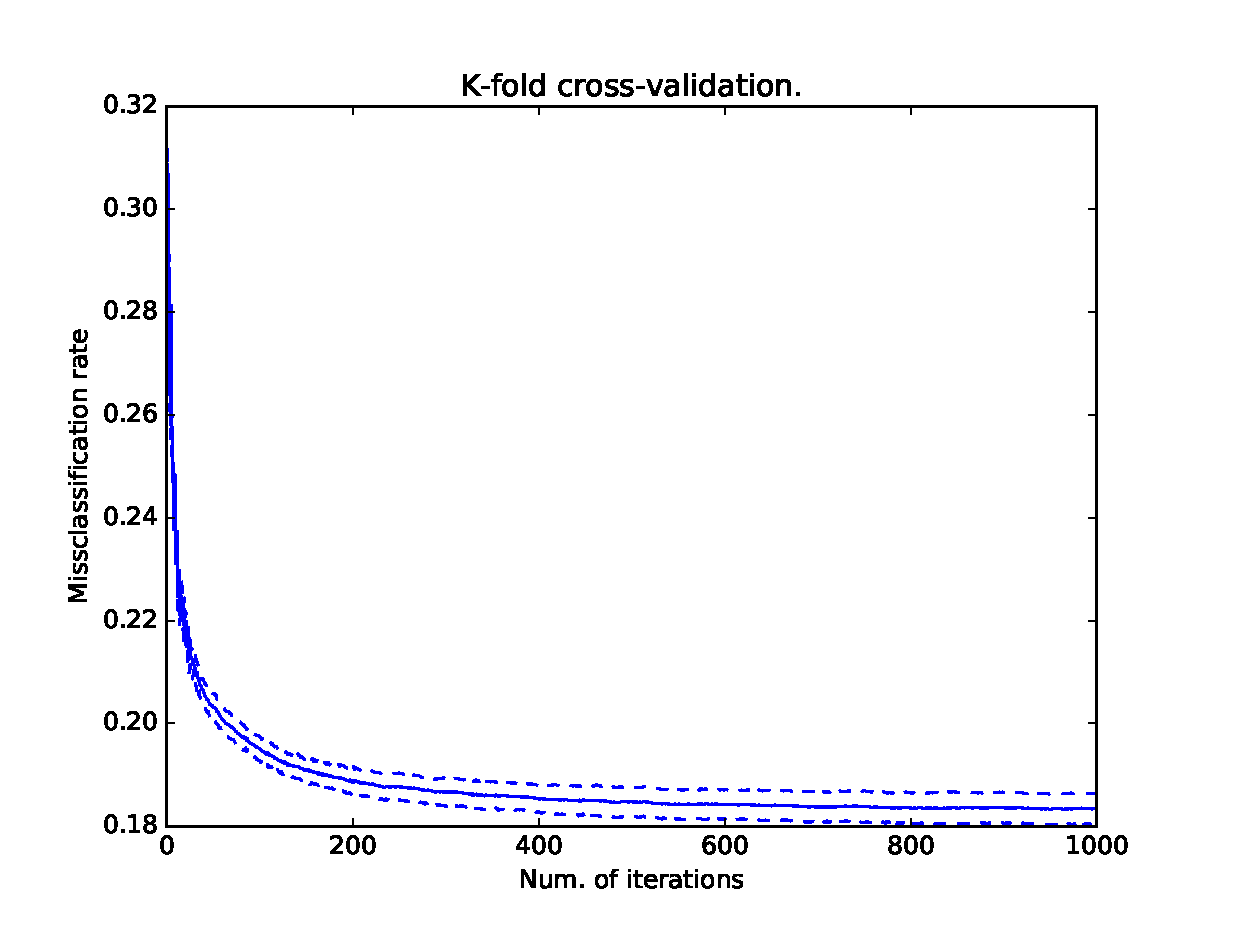
\includegraphics[width=0.58\textwidth]{pics/ada_cv10.eps}
\caption{\label{fig:orgparagraph1}
Missclassification rate with respect to number of stages. 10-fold cross-validation}
\end{figure}


\bibliographystyle{ieeetr}
\bibliography{refs}
\printbibliography
\end{document}